\documentclass{beamer}
\usetheme{Darmstadt}

\usepackage{tikz}

\usepackage{filecontents}
\usepackage{pgfplots, pgfplotstable}
\usepgfplotslibrary{statistics}
\usepackage{graphicx}
\usepackage{appendixnumberbeamer}

\usepackage[utf8]{inputenc}
\usepackage{color}
\usepackage{hyperref}

\bibliographystyle{unsrtnat}
\usepackage[sort&compress,square]{natbib}

\usepackage{csquotes}

% für Listings
\usepackage{listings}
\lstset{numbers=left, numberstyle=\tiny, numbersep=5pt, keywordstyle=\color{black}\bfseries, stringstyle=\ttfamily,showstringspaces=false,basicstyle=\footnotesize,captionpos=b}
\lstset{
	frame=none,
	xleftmargin=2pt,
	stepnumber=1,
	numbers=left,
	numbersep=5pt,
	numberstyle=\ttfamily\tiny\color[gray]{0.3},
	belowcaptionskip=\bigskipamount,
	captionpos=b,
	escapeinside={*'}{'*},
	language=haskell,
	tabsize=2,
	emphstyle={\bf},
	commentstyle=\it,
	stringstyle=\mdseries\rmfamily,
	showspaces=false,
	keywordstyle=\bfseries\rmfamily,
	columns=flexible,
	basicstyle=\small\sffamily,
	showstringspaces=false,
	morecomment=[l]\%,
}

\newcommand{\frbreak}{
	\vfill
	\framebreak
}

\renewcommand{\cite}[1]{\citep{#1}}

\newcommand{\citHughes}{\citep{HughesArrows}}

\newcommand{\code}[1]{\lstinline{#1}}

\newcommand{\fixme}[1]{\colorbox{red}{#1}}

\newcommand{\centeredHeadline}[1]{
\begin{tikzpicture}[overlay, remember picture]
\node[anchor=center] at (current page.center) {
	#1
};
\end{tikzpicture}
}

\title{Building a Parallel Haskell based on Arrows}
\author{Martin Braun}
\date{February 2, 2017}

\setcounter{tocdepth}{2}
\AtBeginSection{\begin{frame} 
\tableofcontents[currentsection]
\end{frame}}
\begin{document}
	\begin{frame}[fragile]
		\centering
		\vspace{0.75cm}
		{\huge\bfseries Arrows for\\Parallel Computation\par}
		\vspace{0.5cm}
		{\Large\itshape Martin Braun\par}
		~\\
		University of Bayreuth\\
		martinbraun123@aol.com
		\vspace{0.5cm}
		
		\vfill
		
		% Bottom of the page
		{\large January 24, 2018\par}
	\end{frame}
	\begin{frame}
		\tableofcontents
	\end{frame}
	%\subsection{Monads}
\begin{frame}[fragile]{Monad Definition}
\begin{lstlisting}[frame=htrbl]
class Monad m where
	(>>=) :: m a -> (a -> m b) -> m b
	return :: a -> m a
\end{lstlisting}

Similar to Java's Optional, we have \code{Maybe a}:
\begin{lstlisting}[frame=htrbl]
instance Monad Maybe where
	(Just a) >>= f = f a
	Nothing >>= _ = Nothing
	return a = Just a
\end{lstlisting}

$\Rightarrow$ composable computation descriptions

\end{frame}

\begin{frame}[fragile]{Monad Usage}
With monadic functions like
\begin{lstlisting}[frame=htrbl]
func :: Int -> Maybe Int
func x
	| x < 0 = Nothing
	| otherwise = Just (x * 2)
\end{lstlisting}
we can compose computations:
\begin{lstlisting}[frame=htrbl]
complicatedFunc :: Int -> Maybe Int
complicatedFunc x = (return x) >>= func >>= ...
\end{lstlisting}
\end{frame}
	\section{Arrows 101}
	\begin{figure}[t]
\centering
\begin{code}
class Arrow arr where
  arr :: (a -> b) -> arr a b
  (>>>) :: arr a b -> arr b c -> arr a c
  first :: arr a b -> arr (a,c) (b,c)

instance Arrow (->) where
	arr f = f
	f >>> g = g . f
	first f = \(a, c) -> (f a, c) 

data Kleisli m a b = Kleisli { run :: a -> m b }

instance Monad m => Arrow (Kleisli m) where
	arr f = Kleisli (return . f)
	f >>> g = Kleisli (\a -> f a >>= g)
	first f = Kleisli (\(a,c) -> f a >>= \b -> return (b,c))
\end{code}
\vfill
\caption{The definition of the |Arrow| type class and its two most typical instances.}
\label{fig:ArrowDefinition}
\end{figure}

\begin{figure}[t]
\centering
\parbox[c][17em]{0.49\linewidth}{%
\vfill
\centering
	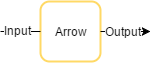
\includegraphics{images/arrow}
\vfill
%	\caption{Schematic depiction of an Arrow.}
%\label{fig:arrow-sch}
}
\parbox[c][17em]{0.49\linewidth}{%
\vfill
\centering
	{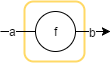
\includegraphics[scale=0.6]{images/arr}}
	{\includegraphics[scale=0.6]{images/compose}}
	{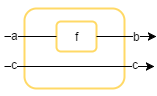
\includegraphics[scale=0.6]{images/first}}
\vfill
%\caption{Schematic depiction of |Arrow| combinators |arr|, |>>>| and |first|.}
%\label{fig:arrows-viz}
}
\caption{Schematic depiction of  an Arrow (left) and its basic
  combinators |arr|, |>>>| and |first| (right).}
\label{fig:arrow-sch}
\label{fig:arrows-viz}
\end{figure}

\subsection{Arrows}
\label{sec:arrows}
Arrows were introduced by \citet{HughesArrows} as a general interface for computation. An Arrow |arr a b| represents  a computation that converts an input |a| to an output |b|. This is defined in the |Arrow| type class shown in Fig.~\ref{fig:ArrowDefinition}.
%
To lift an ordinary function to an Arrow, |arr| is used, analogous to the monadic |return|. Similarly, the composition operator |>>>| is analogous to the monadic composition |>>=| and combines two arrows |arr a b| and |arr b c| by \enquote{wiring} the outputs of the first to the inputs to the second to get a new arrow |arr a c|. Lastly, the |first| operator takes the input Arrow |arr a b| and converts it into an arrow on pairs |arr (a, c) (b, c)| that leaves the second argument untouched. It allows us to to save input across arrows. Figure~\ref{fig:arrows-viz} shows a graphical representation of these basic Arrow combinators.
The most prominent instances of this interface are regular functions |(->)|
and the Kleisli type (Fig.~\ref{fig:ArrowDefinition}), which wraps monadic functions, e.g.  |a -> m b| (with |m| being a Monad).

\begin{figure}[h]
	\centering
	\begin{tabular}{cc}
		% \subcaptionbox
{\label{t1}}{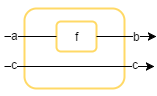
\includegraphics[width = 1.5in]{images/first}} &
		% \subcaptionbox
{\label{fig:secondImg}}{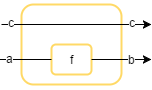
\includegraphics[width = 1.5in]{images/second}} \\
|first| & |second| \\
\midrule
		% \subcaptionbox
{}{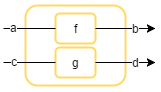
\includegraphics[width = 1.5in]{images/starstarstar}} &
		% \subcaptionbox
{}{\includegraphics[width = 1.5in]{images/andandand}}\\
|(***)|\label{fig:***Img} & |(&&&)| \label{fig:&&&Img} \\
	\end{tabular}
	\caption{Visual depiction of syntactic sugar for Arrows.}
	\label{fig:syntacticSugarArrows}
\end{figure}
Hughes also defined some syntactic sugar (Fig.~\ref{fig:syntacticSugarArrows}): |second|, |***| and |&&&|. 
|second| is the mirrored version of |first| (Appendix~\ref{utilfns}).
|***| combines |first| and |second| to handle two inputs in one arrow, and is defined as follows:
% \begin{figure}[h]
\begin{code}
(***) :: Arrow arr => arr a b -> arr c d -> arr (a, c) (b, d)
f *** g = first f >>> second g
\end{code}
% \caption{The (***) combinator}
% \label{fig:***}
% \end{figure}
The |&&&| combinator, which constructs an Arrow that outputs two different values like |***|, but takes only one input, is:
% \begin{figure}[h]
\begin{code}
(&&&) :: Arrow arr => arr a b -> arr a c -> arr a (b, c)
f &&& g = arr (\a -> (a, a)) >>> (f *** g)
\end{code}
% \caption{The (\&\&\&) combinator}
% \label{fig:&&&}
% \end{figure}
A~first short example given by Hughes on how to use arrows is addition with arrows:
%|add| over arrows, which can be seen in Fig.~\ref{fig:addArrows}.
% \begin{figure}[h]
\begin{code}
add :: Arrow arr => arr a Int -> arr a Int -> arr a Int
add f g = (f &&& g) >>> arr (\(u, v) -> u + v)
\end{code}
% \caption{Add over arrows}
% \label{fig:addArrows}
% \end{figure}
% The benefit of using the |Arrow| typeclass is that any type which is shown to be an arrow can be used in conjunction with this newly created |add| combinator. Even though this example is quite simple, the power of the arrow interface immediately is clear: If a type is an arrow, it can automatically used together with every library that works on arrows. Compared to simple Monads, this enables us to write code that is more extensible, without touching the internals of the specific arrows.
% \\\\
% \textit{Note: In the definitions Hughes gave in his paper, the notation |a b c| for an arrow from |b| to |c| is used. We use the equivalent definition |arr a b| for an arrow from |a| to |b| instead, to make it easier to find the arrow type in type signatures.}
%

The more restrictive interface of Arrows allows for more elaborate composition and transformation combinators---a Monad can be \emph{anything}, an Arrow is a process of doing something, a \emph{computation}. This is exactly one of the key challenges in parallel computing.


%%% Local Variables:
%%% mode: latex
%%% TeX-master: "main"
%%% End:

	\section{Background}
\label{sec:background}
\subsection{Short introduction to parallel Haskells}
There are already several ways to write parallel programs in Haskell. As we will base our parallel arrows on existing parallel Haskells, we will now give a short introduction to the ones we use as backends in this paper.

In its purest form, parallel computation (on functions) can be looked at as the execution of some functions \inlinecode{a -> b} in parallel:

\begin{figure}[h]
%\begin{lstlisting}[frame=htrbl]
\begin{code}
parEvalN :: [a -> b] -> [a] -> [b]
\end{code}
%\end{lstlisting}
\caption{parEvalN's type signature}
\label{fig:parEvalNTypeSig}
\end{figure}
\begin{figure}[h]
	\includegraphics[scale=0.7]{images/parEvalN}
	\caption{Schematic illustration of parEvalN}
	\label{fig:parEvalN}
\end{figure}
\olcomment{make them to real figures? with environment, reference and such?}
Before we go into detail on how we can use this idea of parallelism for parallel Arrows, as a short introduction to parallelism in Haskell we will now implement \inlinecode{parEvalN} with several different parallel Haskells.

\subsubsection{Multicore Haskell}
Multicore Haskell \cite{Marlow2009,Trinder1999} is way to do parallel processing found in standard GHC.\footnote{Multicore Haskell on Hackage is available under \url{https://hackage.haskell.org/package/parallel-3.2.1.0}, compiler support is integrated in the stock GHC.} It ships with parallel evaluation strategies \cite{Trinder1998a,Marlow2010} for several types which can be applied with \inlinecode{using :: a -> Strategy a -> a}. For \inlinecode{parEvalN} this means that we can just apply the list of functions \inlinecode{[a -> b]} to the list of inputs \inlinecode{[a]} by zipping them with the application operator \inlinecode{\$}. We then evaluate this lazy list \inlinecode{[b]} according to a \inlinecode{Strategy [b]} with the \inlinecode{using :: a -> Strategy a -> a} operator. We construct this strategy with \inlinecode{parList :: Strategy a -> Strategy [a]} and \inlinecode{rdeepseq :: NFData a => Strategy a} where the latter is a strategy which evalutes to normal form. To ensure that programs that use \inlinecode{parEvalN} have the correct evaluation order, we annotate the computation with \inlinecode{pseq :: a -> b -> b} which forces the compiler to not reorder multiple \inlinecode{parEvalN} computations. This is particularly necessary in circular communication topologies like in the \inlinecode{torus} or \inlinecode{ring} skeleton that we will see in chapter \ref{sec:topology-skeletons} which resulted in deadlock scenarios when executed without \inlinecode{pseq} during testing for this paper.

\begin{lstlisting}[frame=htrbl]
parEvalN :: (NFData b) => [a -> b] -> [a] -> [b]
parEvalN fs as = let bs = zipWith ($) fs as in
	(bs `using` parList rdeepseq) `pseq` bs
\end{lstlisting}
\begin{figure}[h]
	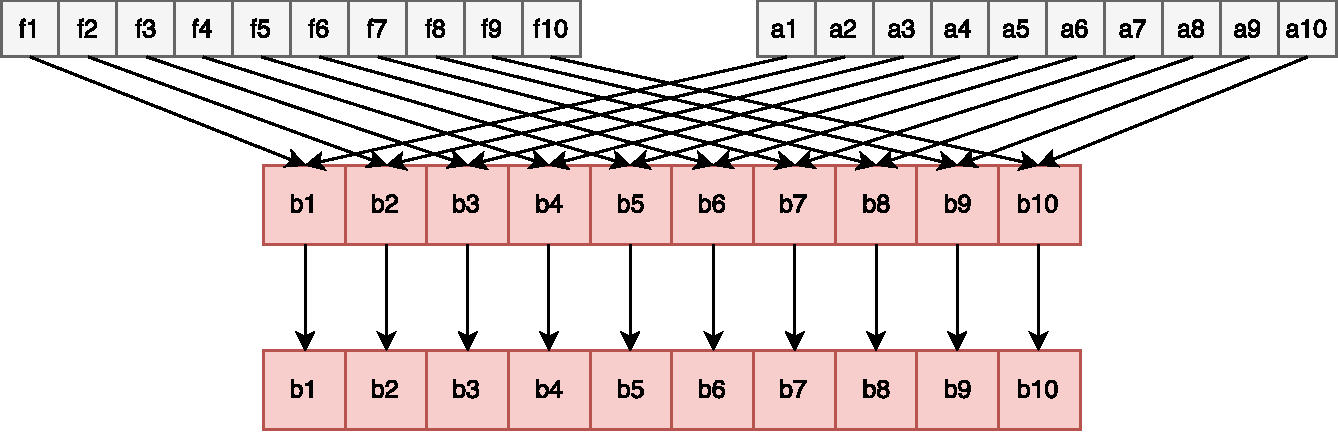
\includegraphics[scale=0.5]{images/parEvalNMulticore}
	\caption{Dataflow of the Multicore Haskell parEvalN version}
\end{figure} %$ %% formatting

\subsubsection{ParMonad}
The \inlinecode{Par} monad\footnote{It can be found in the \texttt{monad-par} package on hackage under \url{https://hackage.haskell.org/package/monad-par-0.3.4.8/}.} introduced by \citet{monad_par_paper_2011}, is a monad designed for composition of parallel programs.


Our parallel evaluation function \inlinecode{parEvalN} can be defined by zipping the list of \inlinecode{[a -> b]} with the list of inputs \inlinecode{[a]} with the application operator \inlinecode{\$} just like with Multicore Haskell. Then, we map over this not yet evaluated lazy list of results \inlinecode{[b]} with \inlinecode{spawnP :: NFData a => a -> Par (IVar a)} to transform them to a list of not yet evaluated forked away computations \inlinecode{[Par (IVar b)]}, which we convert to \inlinecode{Par [IVar b]} with \inlinecode{sequenceA}. We wait for the computations to finish by mapping over the \inlinecode{IVar b}'s inside the \inlinecode{Par} monad with \inlinecode{get}. This results in \inlinecode{Par [b]}. We finally execute this process with \inlinecode{runPar} to finally get \inlinecode{[b]} again.

\textbf{\textcolor{red}{explain problems with laziness here. Problems with torus}}

\begin{lstlisting}[frame=htrbl]
parEvalN :: (NFData b) => [a -> b] -> [a] -> [b]
parEvalN fs as = runPar $ 
	(sequenceA $ map (spawnP) $ zipWith ($) fs as) >>= mapM get
\end{lstlisting}
\begin{figure}[h]
	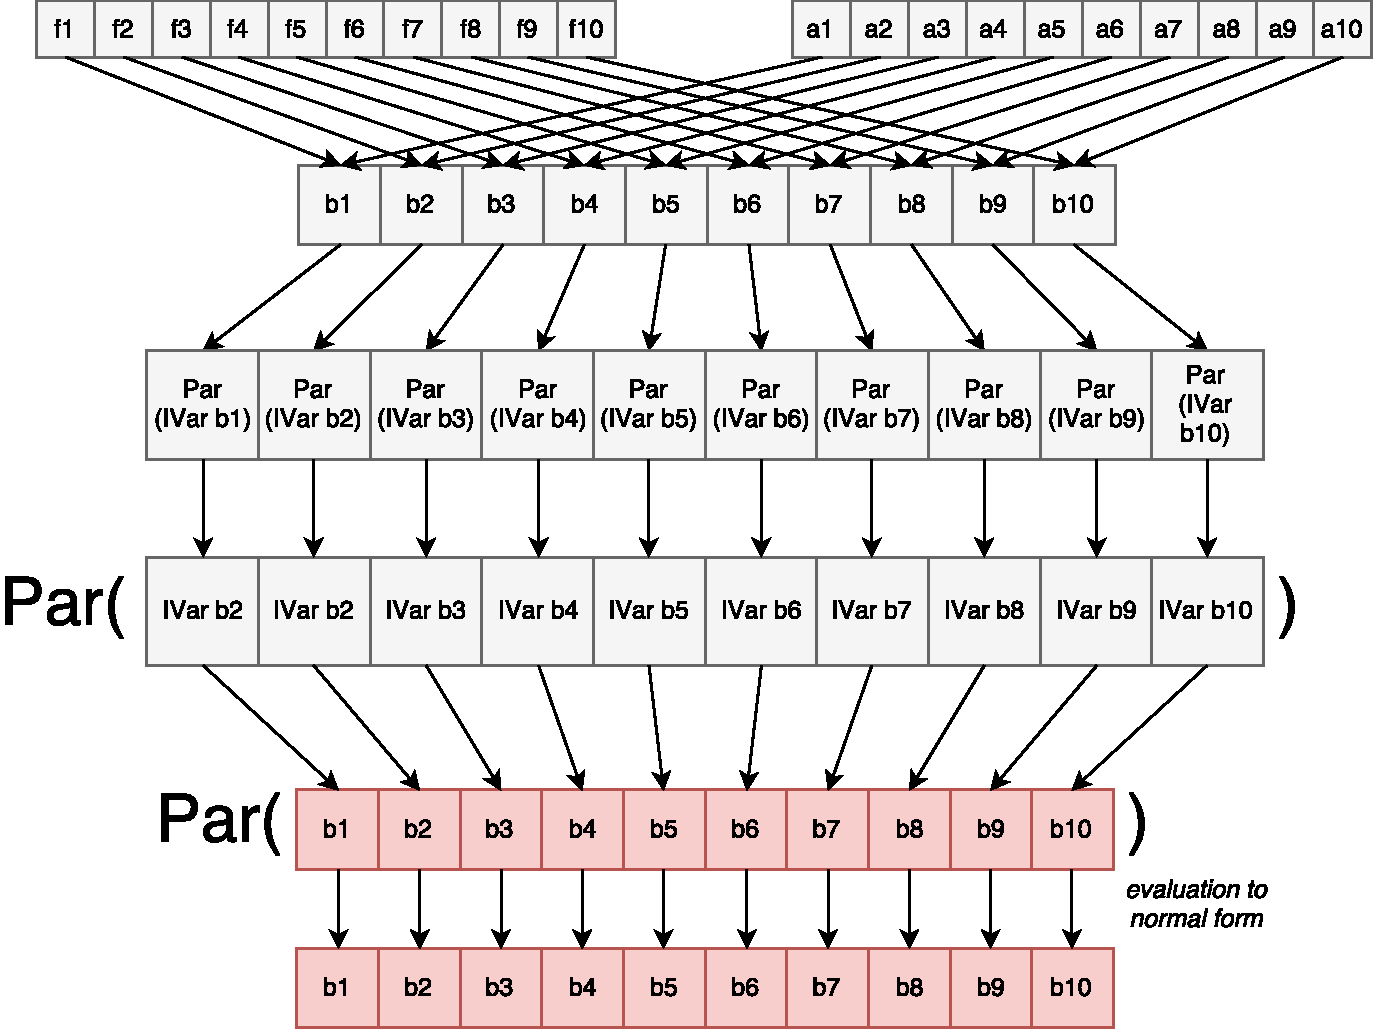
\includegraphics[scale=0.5]{images/parEvalNParMonad}
	\caption{Dataflow of the Par Monad parEvalN version}
\end{figure}

\subsubsection{Eden}
Eden \cite{eden,Loogen2012} is a parallel Haskell for distributed memory and comes with a MPI and a PVM backends.\footnote{See also \url{http://www.mathematik.uni-marburg.de/~eden/} and \url{https://hackage.haskell.org/package/edenmodules-1.2.0.0/}.} This means that it works on clusters as well so it makes sense to have a Eden-based backend for our new parallel Haskell flavour.

Eden was designed to work on clusters, but with a further simple backend it operates on multicores. However, in contrast to many other parallel Haskells, in Eden each process has its own heap. This seems to be a waste of memory, but with distributed programming paradigm and individual GC per process, Eden yields good performance results also on multicores \cite{arcs-dc,aswad2009low}.

While Eden also comes with a monad \inlinecode{PA} for parallel evaluation, it also ships with a completely functional interface that includes
%\\
%\inlinecode{spawnF :: (Trans a, Trans b) => [a -> b] -> [a] -> [b]}.
%\\
a \inlinecode{spawnF} function that
%This 
allows us to define \inlinecode{parEvalN} directly:

\begin{lstlisting}[frame=htrbl]
parEvalN :: (Trans a, Trans b) => [a -> b] -> [a] -> [b]
parEvalN = spawnF 
\end{lstlisting}
\begin{figure}[h]
	\includegraphics[scale=0.5]{images/parEvalNEden}
	\caption{Dataflow of the Eden parEvalN version}
\end{figure}

\paragraph{Eden TraceViewer.}
To comprehend the efficiency and the lack thereof in a parallel program, an inspection of its execution is extremely helpful. While some large-scale solutions exist \cite{Geimer2010}, the parallel Haskell community mainly utilises the tools Threadscope \cite{Wheeler2009} and Eden TraceViewer\footnote{See ..... on hackage for the last available version of Eden TraceViewer. There was an effort to implement the TraceViewer using modern web technologies \cite{traceviewer-web}.} \cite{Berthold2007a}. In the next sections we will present some \emph{traces}, the post-mortem process diagrams of Eden processes and their activity.

In a trace, the $x$ axis shows the time, the $y$ axis enumerates the machines and processes. A~trace shows a running process in green, a blocked process is red. If the process is \enquote{runnable}, \ie it may run, but does not, it is yellow. The typical reason for then is GC. An inactive machine where no processes are started yet, or all are already terminated, is shows as a blue bar. A~comminication from one process to another is represented with a black arrow. A~stream of communications, \eg a transmitted list is shows as a dark shading between sender and receiver processes.

\olcomment{show example trace or refer to a trace in later figures}


%%% Local Variables:
%%% mode: latex
%%% TeX-master: "main"
%%% End:

	\section{Parallel Arrows}
We have seen what Arrows are and how they can be seen as a general interface to computation. In the following section we will discuss how Arrows can also be seen as a general interface not only to computation, but to \textbf{parallel computation} as well. We start by introducing the interface and explaining the reasonings behind it. Then, we discuss some implementations using exisiting parallel Haskells. Finally, we explain why using Arrows for expressing parallelism is beneficial.
\subsection{The ArrowParallel interface}
In its purest form, parallel computation (on functions) can be looked at as the execution of some functions \code{a -> b} in parallel:
\begin{lstlisting}[frame=htrbl]
parEvalN :: [a -> b] -> [a] -> [b]
\end{lstlisting}
Translating this into arrow terms gives us a new operator \code{parEvalN} that lifts a list of arrows \code{[arr a b]} to a parallel arrow \code{arr [a] [b]} (This combinator is similar to our utility function listApp, but does parallel instead of serial evaluation).
\begin{lstlisting}[frame=htrbl]
parEvalN :: (Arrow arr) => [arr a b] -> arr [a] [b]
\end{lstlisting}
With this definition of \code{parEvalN}, parallel execution can be looked at as yet another arrow combinator. But as the implementation may differ depending on the actuall type of the arrow \code{arr} and we want this to be an interface for different backends, we have to introduce the new typeclass \code{ArrowParallel} to host this combinator.
\begin{lstlisting}[frame=htrbl]
class Arrow arr => ArrowParallel arr a b where
	parEvalN :: [arr a b] -> arr [a] [b]
\end{lstlisting}
Sometimes parallel Haskells require additional configuration parameters for information about the execution environment. This is why we also introduce an additional \code{conf} parameter to the function. We also do not want \code{conf} to be of a fixed type, as the configuration parameters can differ for different instances of \code{ArrowParallel}, so we add it to the type signature of the typeclass as well.
\begin{lstlisting}[frame=htrbl]
class Arrow arr => ArrowParallel arr a b conf where
	parEvalN :: conf -> [arr a b] -> arr [a] [b]
\end{lstlisting}
We don't require the conf parameter in every implementation. If it is not needed, we usually want to allow the \code{conf} type parameter to be of any type and don't even evaluate it by blanking it in the type signature of the implemented \code{parEvalN} as we will see in the implementation sections.

\subsection{Multicore Haskell}
The Multicore Haskell implementation of this class is straightforward using listApp from \ref{utilfns} combined with the \code{using} operator from Multicore Haskell.
\begin{lstlisting}[frame=htrbl]
instance (NFData b, ArrowApply arr, ArrowChoice arr) =>
	ArrowParallel arr a b conf where
		parEvalN _ fs = listApp fs >>> arr (flip using $ parList rdeepseq)
\end{lstlisting}
We hardcode the \code{parList rdeepseq} strategy here as in this context it is the only one making sense as we usually want the output list to be fully evaluated to its normal form.

\subsection{ParMonad}
The ParMonad implementation makes use of Haskells laziness and ParMonad's \code{spawnP :: a -> Par (IVar a)} function which forks away the computation of a value and returns an IVar containing the result in the Par monad.
\\\\
We therefore apply each function to its corresponding input value with \code{app} and then fork the computation away with \code{arr spawnP} inside a \code{zipWithArr} call. This yields a list \code{[Par (IVar b)]}, which we then convert into \code{Par [IVar b]} with \code{arr sequenceA}. In order to wait for the computation to finish, we map over the \code{IVar}s inside the ParMonad with \code{arr (>>= mapM get)}. The result of this operation is a \code{Par [b]} from which we can finally remove the monad again by running \code{arr runPar} to get our output of \code{[b]}.
\begin{lstlisting}[frame=htrbl]
instance (NFData b, ArrowApply arr, ArrowChoice arr) =>
	ArrowParallel arr a b conf where
		parEvalN _ fs = 
			(arr $ \as -> (fs, as)) >>>
			zipWithArr (app >>> arr spawnP) >>>
			arr sequenceA >>>
			arr (>>= mapM get) >>>
			arr runPar
\end{lstlisting}

\subsection{Eden}
For the Multicore and ParMonad implementation we could use general implementations that just required the \code{ArrowApply} and \code{ArrowChoice} typeclasses. With Eden this is not the case as we can only spawn a list of functions and we cannot extract simple functions out of arrows. While we could still manage to have only one class in the module by introducing a typeclass like
\begin{lstlisting}[frame=htrbl]
class (Arrow arr) => ArrowUnwrap arr where
	arr a b -> (a -> b)
\end{lstlisting}
we don't do this in this paper, as this seems too hacky. For now, we just implement \code{ArrowParallel} for normal functions
\begin{lstlisting}[frame=htrbl]
instance (Trans a, Trans b) => ArrowParallel (->) a b conf where
parEvalN _ fs as = spawnF fs as
\end{lstlisting}
and the Kleisli type.
\begin{lstlisting}[frame=htrbl]
instance (Monad m, Trans a, Trans b, Trans (m b)) =>
	ArrowParallel (Kleisli m) a b conf where
parEvalN conf fs =
	(arr $ parEvalN conf (map (\(Kleisli f) -> f) fs)) >>>
	(Kleisli $ sequence)
\end{lstlisting}

\subsection{HdpH}

\subsection{Benefits of parallel Arrows}
We have seen that we can wrap parallel Haskells inside of the \code{ArrowParallel} interface, but why do we abstract parallelism this way and what does this approach do better than the other parallel Haskells?
\begin{itemize}
	\item \textbf{Arrow API benefits}:
	With the \code{ArrowParallel} typeclass we do not lose any benefits of using arrows as \code{parEvalN} is just yet another arrow combinator. The resulting arrow can be used in the same way its serial version can be used. This is a big advantage of this approach, especially compared to the monad solutions as all arrow combinators will continue to work instead of requiring special ones for each parallel monad.
	\item \textbf{Abstraction}:
	With the \code{ArrowParallel} typeclass, we abstracted all parallel implementation logic away from the business logic. This gives us the beautiful situation of being able to write our code against the interface the typeclass gives us without being bound to any parallel Haskell. So as an example, during development, we can run the code on the simple Multicore version and afterwards deploy it on a cluster using an Eden built, by just swapping out the actual \code{ArrowParallel} instance.
\end{itemize}

	%\section{Utility Functions}\label{utilfns}
\subsection{mapArr}
The mapArr combinator lifts any arrow \code{arr a b} to an arrow \code{arr [a] [b]} \cite{programming_with_arrows},
\begin{lstlisting}[frame=htrbl]
mapArr :: ArrowChoice arr => arr a b -> arr [a] [b]
mapArr f =
	arr listcase >>>
	arr (const []) ||| (f *** mapArr f >>> arr (uncurry (:)))
	where
		listcase [] = Left ()
		listcase (x:xs) = Right (x,xs)
\end{lstlisting}
with
\begin{lstlisting}[frame=htrbl]
(|||) :: ArrowChoice arr a c -> arr b c -> arr (Either a b) c
\end{lstlisting}
%It takes two arrows \code{arr a c} and \code{arr b c} and combines them into a new arrow \code{arr (Either a b) c} which pipes all \code{Left a}'s to the first arrow and all \code{Right b}'s to the second arrow.
\frbreak

\subsection{zipWithArr \& listApp}
zipWithArr lifts any arrow \code{arr (a, b) c} to an arrow \code{arr ([a], [b]) [c]}:
\begin{lstlisting}[frame=htrbl]
zipWithArr :: ArrowChoice arr => arr (a, b) c -> arr ([a], [b]) [c]
zipWithArr f = (arr $ \(as, bs) -> zipWith (,) as bs) >>>
	mapArr f
\end{lstlisting}
listApp converts a list of arrows \code{[arr a b]} to a new arrow \code{arr [a] [b]}:
\begin{lstlisting}[frame=htrbl]
listApp :: (ArrowChoice arr, ArrowApply arr) =>
	[arr a b] -> arr [a] [b]
listApp fs = (arr $ \as -> (fs, as)) >>> zipWithArr app
\end{lstlisting}
with the \code{ArrowApply} that defines \code{app :: arr (arr a b, a) c}.

	\subsection{ArrowParallel Implementations}
\begin{frame}[fragile]{GpH}
\begin{lstlisting}[frame=htrbl]
data Conf a = Conf (Strategy a)

instance (ArrowChoice arr) =>
  ArrowParallel arr a b (Conf b) where
    parEvalN (Conf strat) fs =
        evalN fs >>>
        arr (withStrategy (parList strat))
\end{lstlisting}
\begin{center}
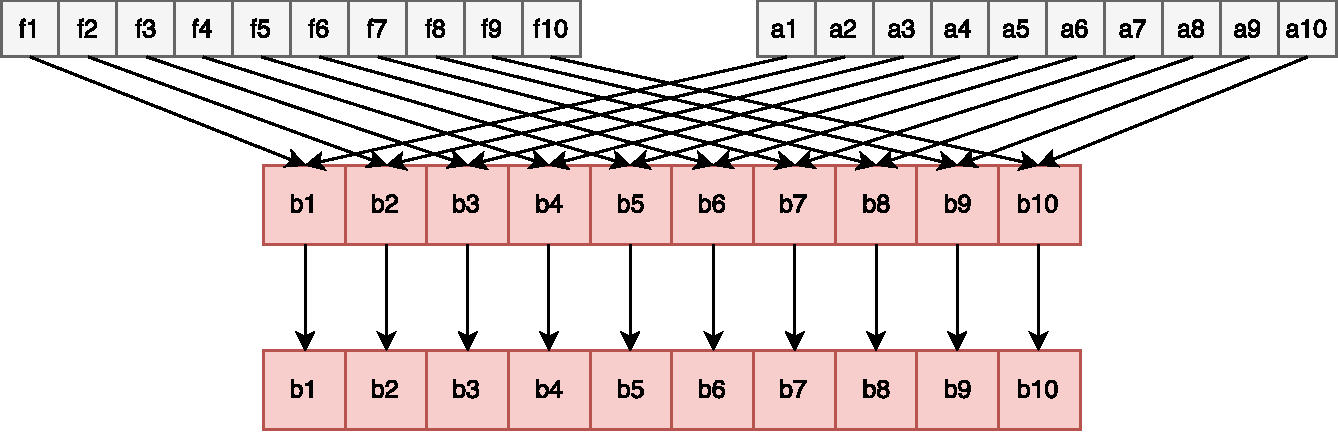
\includegraphics[scale=0.45]{images/parEvalNMulticore}
\end{center}
\end{frame}

\begin{frame}[fragile]{ParMonad}
\begin{lstlisting}[frame=htrbl]
type Strategy a = a -> Par (IVar a)
data Conf a = Conf (Strategy a)

instance (ArrowChoice arr) => ArrowParallel arr a b (Conf b) where
    parEvalN (Conf strat) fs =
        evalN (map (>>> arr strat) fs) >>>
        ...
\end{lstlisting}
\begin{center}
\includegraphics[scale=0.4]{images/parEvalNParMonad1}
\end{center}
\end{frame}

\begin{frame}[fragile]{ParMonad}
\begin{lstlisting}[frame=htrbl]
        ...
        arr sequenceA >>>
        arr (>>= mapM Control.Monad.Par.get) >>>
        arr runPar
\end{lstlisting}
\begin{center}
\includegraphics[scale=0.4]{images/parEvalNParMonad2}
\end{center}
\end{frame}


\begin{frame}[fragile]{Eden problems}
For Eden we need separate implementations.\\~\\
This is because of \code{spawnF} only supporting functions \lstinline{(->)}:
\begin{lstlisting}[frame=htrbl]
spawnF :: (Trans a, Trans b) => [a -> b] -> [a] -> [b]
\end{lstlisting}
\pause
Hacky alternative:
\begin{lstlisting}[frame=htrbl]
class (Arrow arr) => ArrowUnwrap arr where
    arr a b -> (a -> b)
\end{lstlisting}
\end{frame}

\begin{frame}[fragile]{Eden implementation - Functions}
Straightforward:
\begin{lstlisting}[frame=htrbl]
data Conf = Nil

instance (Trans a, Trans b) => ArrowParallel (->) a b conf where
	parEvalN _ = spawnF
\end{lstlisting}
\begin{center}
\includegraphics[scale=0.5]{images/parEvalNEden}
\end{center}
\end{frame}

\begin{frame}[fragile]{Eden implementation - Kleisli}
Implementation for the Kleisli Type:
\begin{lstlisting}[frame=htrbl]
instance (ArrowParallel (->) a (m b) Conf,
  Monad m, Trans a, Trans b, Trans (m b)) =>
  ArrowParallel (Kleisli m) a b conf where
    parEvalN conf fs = 
      arr (parEvalN conf (map (\(Kleisli f) -> f) fs)) >>>
      Kleisli sequence
\end{lstlisting}
\begin{center}
\includegraphics[scale=0.5]{images/parEvalNEden}
\end{center}
\end{frame}
	\section{Usability}
	\subsubsection{Syntactic Sugar} \label{syntacticSugar}
For basic arrows, we have the \inlinecode{(***)} combinator (Fig.~\ref{fig:***Img},~\ref{fig:***}) which allows us to combine two arrows \inlinecode{arr a b} and \inlinecode{arr c d} into an arrow \inlinecode{arr (a, c) (b, d)} which does both computations at once. This can easily be translated into a parallel version \inlinecode{(|***|)} (Fig.~\ref{fig:|***|}) with the use of \inlinecode{parEval2}, but for this we require a backend which has an implementation that does not require any configuration (hence the \inlinecode{()} as the conf parameter in Fig.~\ref{fig:|***|}).
\begin{figure}[h]
\begin{lstlisting}[frame=htrbl]
(|***|) :: (ArrowChoice arr, ArrowParallel arr (Either a c) (Either b d) ())) =>
	arr a b -> arr c d -> arr (a, c) (b, d)
(|***|) = parEval2 ()
\end{lstlisting}
\caption{Definition of (|***|) - the parallel version of (***)}
\label{fig:|***|}
\end{figure}
% With this we can analogously to the serial \inlinecode{&&&}
We define the parallel \inlinecode{(|\&\&\&|)} (Fig.~\ref{fig:|&&&|}) in a similar manner to its sequential pendant \inlinecode{(\&\&\&)} (Fig.~\ref{fig:&&&Img},~\ref{fig:&&&}).
\begin{figure}[h]
\begin{lstlisting}[frame=htrbl]
(|&&&|) :: (ArrowChoice arr, ArrowParallel arr (Either a a) (Either b c) ()) =>
	arr a b -> arr a c -> arr a (b, c)
(|&&&|) f g = (arr $ \a -> (a, a)) >>> f |***| g
\end{lstlisting} % $ %% formatting
\caption{Definition of (|\&\&\&|) - the parallel version of (\&\&\&)}
\label{fig:|&&&|}
\end{figure}
	\subsection{Map Skeletons}
\begin{frame}[fragile]{Map Skeletons (1)}
parEvalN, but \textbf{chunky}:
\begin{lstlisting}[frame=htrbl]
parEvalNLazy :: conf -> ChunkSize -> [arr a b] -> arr [a] [b]
\end{lstlisting}
\begin{center}
\includegraphics[scale=0.5]{images/parEvalNLazy}
\end{center}
parallel evaluation of \textbf{different typed functions}:
\begin{lstlisting}[frame=htrbl]
parEval2 :: conf -> arr a b -> arr c d -> arr (a, c) (b, d)
\end{lstlisting}
\begin{center}
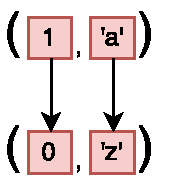
\includegraphics[scale=0.5]{images/parEval2}
\end{center}
\end{frame}
\begin{frame}[fragile] {Map Skeletons (2)}
map, but in \textbf{parallel}:
\begin{lstlisting}[frame=htrbl]
parMap :: conf -> arr a b -> arr [a] [b]
\end{lstlisting}
\begin{center}
\includegraphics[scale=0.5]{images/parMap}
\end{center}
parMap, but \textbf{chunky}:
\begin{lstlisting}[frame=htrbl]
parMapStream :: conf -> ChunkSize -> arr a b -> arr [a] [b]
\end{lstlisting}
\begin{center}
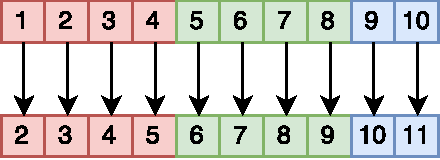
\includegraphics[scale=0.5]{images/parMapStream}
\end{center}
\end{frame}
\begin{frame}[fragile]{Map Skeletons (3)}
parMap, but with \textbf{workload distribution}:
\begin{lstlisting}[frame=htrbl]
farm :: conf -> NumCores -> arr a b -> arr [a] [b]
\end{lstlisting}
\begin{center}
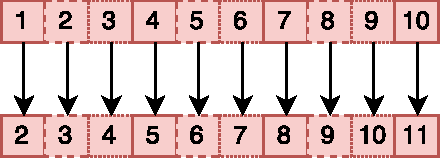
\includegraphics[scale=0.5]{images/farm}
\end{center}
farm, but \textbf{chunky}:
\begin{lstlisting}[frame=htrbl]
farmChunk ::
	conf -> ChunkSize -> NumCores -> arr a b-> arr [a] [b]
\end{lstlisting}
\begin{center}
\includegraphics[scale=0.5]{images/farmChunk}
\end{center}
\end{frame}
	\section{Futures} \label{futures}
Consider the parallel arrow combinator in Fig.~\ref{fig:someCombinator}
\begin{figure}[h]
\begin{code}
someCombinator :: (Arrow arr) => [arr a b] -> [arr b c] -> arr [a] [c]
someCombinator fs1 fs2 = parEvalN () fs1 >>> rightRotate >>> parEvalN () fs2
\end{code}
\caption{An example parallel Arrow combinator without Futures.}
\label{fig:someCombinator}
\end{figure}
In a distributed environment, a resulting arrow of this combinator first evaluates all |[arr a b]| in parallel, sends the results back to the master node, rotates the input once and then evaluates the |[arr b c]| in parallel to then gather the input once again on the master node.
Such situations arise, \eg in scientific computations when the data distributed across the nodes needs to be transposed. A concrete example is 2D FFT computation \cite{Gorlatch,Berthold2009-fft}.

While the example in Fig.~\ref{fig:someCombinator} could be rewritten into only one |parEvalN| call by directly wiring the arrows properly together, this example illustrates an important problem: When using a |ArrowParallel| backend that resides on multiple computers, all communication between the nodes is done via the master node, as shown in the Eden trace in Figure~\ref{fig:withoutFutures}. This can become a serious bottleneck %in heavy threaded applications.
for larger amount of data and number of processes \citep[showcases][as, \eg]{Berthold2009-fft}.
\begin{figure}[ht]
	\centering
	\includegraphics[width=0.9\textwidth]{images/withoutFutures}
	\caption[without Futures]{Communication between 4 threads without Futures. All communication goes through the master node. Each bar represents one process. Black lines between processes represent communication. Colors: blue $\hat{=}$ idle, green $\hat{=}$ running, red  $\hat{=}$ blocked, yellow $\hat{=}$ suspended.}
	\label{fig:withoutFutures}
\olcomment{more practical and heavy-weight example! fft (I have the code)?}\\
\mbcomment{Depends... Are the communications easy to read in such an example?}\\
\mbcomment{Keep the description for the different colours, or link to the EdenTV description in \ref{sec:edentv}}
\end{figure}

This motivates for an approach that allows the nodes to communicate directly with each other. Thankfully, Eden, the distributed parallel Haskell we have used in this paper so far, already ships with the concept of |RD| (remote data) that enables this behaviour \cite{AlGo03a,Dieterle2010}.

But as we want code written against our API to be implementation agnostic, we have to wrap this context. We do this with the |Future| typeclass (Fig.~\ref{fig:future}).
\begin{figure}[h]
\begin{code}
class Future fut a | a -> fut where
    put :: (Arrow arr) => arr a (fut a)
    get :: (Arrow arr) => arr (fut a) a
\end{code}
\caption{Definition of the |Future| typeclass.}
\label{fig:future}
\end{figure}
Since |RD| is only a type synonym for communication type that Eden uses internally, we have to use some wrapper classes to fit that definition, though, as seen in Appendix in Fig.~\ref{fig:RDFuture}. This is due to the same reason we had to introduce a wrapper for |Strategy a| in the Multicore Haskell implementation of |ArrowParallel| in Section~\ref{sec:parrows:multicore}.

For our Par Monad and Multicore Haskell backends, we can simply use |MVar|s \cite{jones1996concurrent} (Fig.~\ref{fig:MVarFuture}), because we have shared memory in a single node and don't require Eden's sophisticated communication channels. \fixme{explain MVars}
\begin{figure}[h]
\begin{code}
{-# NOINLINE putUnsafe #-}
putUnsafe :: a -> MVar a
putUnsafe a = unsafePerformIO $ do
    mVar <- newEmptyMVar
    putMVar mVar a
    return mVar

instance (NFData a) => Future MVar a where
    put = arr putUnsafe
    get = arr takeMVar >>> arr unsafePerformIO
\end{code}
\caption{MVar instance of the Future typeclass for the Par Monad and Multicore Haskell backends.}
\label{fig:MVarFuture}
\end{figure} % $

Furthermore, in order for these |Future| types to fit with the |ArrowParallel| instances we gave earlier, we have to give the necessary |NFData| and |Trans| instances, the latter are only needed in Eden. Because |MVar| already ships with a |NFData| instance, we only have to supply two simple instances for our |RemoteData| type:
% \begin{figure}[h]
\begin{code}
instance NFData (RemoteData a) where
    rnf = rnf . rd
instance Trans (RemoteData a)
\end{code}
% \caption{NFData and Trans instances for the RemoteData type. The Trans instance does not have any functions declared as the default implementation suffices here. See \url{https://hackage.haskell.org/package/edenmodules-1.2.0.0/docs/Control-Parallel-Eden.html\#g:5} for more information.}
% \end{figure}
The |Trans| instance does not have any functions declared as the default implementation suffices here.

Going back to our communication example we can use this |Future| concept in order to enable direct communications between the nodes in the following way:
\begin{figure}[h]
\begin{code}
someCombinator :: (Arrow arr) => [arr a b] -> [arr b c] -> arr [a] [c]
someCombinator fs1 fs2 =
	parEvalN () (map (>>> put) fs1) >>>
	rightRotate >>>
	parEvalN () (map (get >>>) fs2)
\end{code}
\caption{The combinator from Fig.~\ref{fig:someCombinator} in parallel.}
\label{fig:someCombinatorParallel}
\end{figure}
In a distributed environment, this gives us a communication scheme with messages going through the master node only if it is needed - similar to what is shown in the trace in Fig.~\ref{fig:withFutures}.\olcomment{Fig.~3 is not really clear. Do Figs 2-3 with a lot of load?}
\begin{figure}[ht]
	\centering
	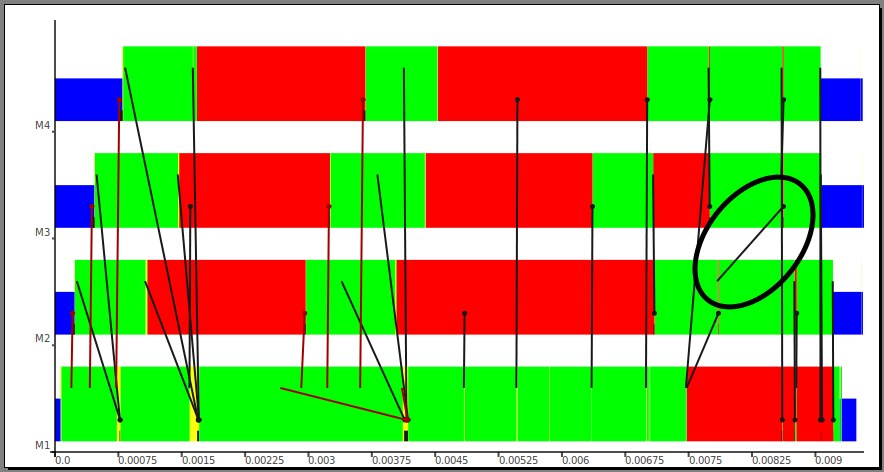
\includegraphics[width=0.9\textwidth]{images/withFutures}
	\caption[with Futures]{Communication between 4 threads with Futures. Other than in Fig.~\ref{fig:withoutFutures}, threads communicate directly (black lines between the bars) instead of always going through the master node (bottom bar).}
	\label{fig:withFutures}
\end{figure}
	%\FloatBarrier
\subsection{Topological skeletons}
\label{sec:topology-skeletons}
Even though many algorithms can be expressed by parallel maps, some problems require more sophisticated skeletons. The Eden library leverages this problem and already comes with more predefined skeletons\footnote{Available on Hackage: \url{https://hackage.haskell.org/package/edenskel-2.1.0.0/docs/Control-Parallel-Eden-Topology.html}.}, among them a |pipe|, a |ring|, and a |torus| implementations \citep{Eden:SkeletonBookChapter02}. These seem like reasonable candidates to be ported to our Arrow-based parallel Haskell. We aim to showcase that we can express more sophisticated skeletons with parallel Arrows as well.

If we used the original definition of |parEvalN|, however, these skeletons would produce an infinite loop with the GpH and |Par| Monad which during runtime would result in the program crash. This materialises with the usage of |loop| of the |ArrowLoop| type class and we think that this is due to difference of how evaluation is done in these backends when compared to Eden. An investigation of why this difference exists is beyond the scope of this work, we only provide a workaround for these types of skeletons as such they probably are not of much importance outside of a distributed memory environment. However our workaround enables users of the DSL to test their code within a shared memory setting.
% even though other skeletons would be better suited to be run with them. --- OL: I don't get this sentence part
The idea of the fix is to provide a |ArrowLoopParallel| type class that has two functions -- |loopParEvalN| and |postLoopParEvalN|, where the first is to be used inside an |loop| construct while the latter will be used right outside of the |loop|. This way we can delegate to the actual |parEvalN| in the spot where the backend supports it.
\begin{code}
class ArrowParallel arr a b conf =>
	ArrowLoopParallel arr a b conf where
    loopParEvalN :: conf -> [arr a b] -> arr [a] [b]
    postLoopParEvalN :: conf -> [arr a b] -> arr [a] [b]
\end{code}
As Eden has no problems with the looping skeletons, we use this instance:
\begin{code}
instance (ArrowChoice arr, ArrowParallel arr a b Conf) =>
	ArrowLoopParallel arr a b Conf where
    loopParEvalN = parEvalN
    postLoopParEvalN _ = evalN
\end{code}
As the backends for the |Par| Monad and GpH have problems with |parEvalN| inside of |loop| their respective instances for |ArrowLoopParallel| look like this:
\begin{code}
instance (ArrowChoice arr, ArrowParallel arr a b (Conf b)) =>
	ArrowLoopParallel arr a b (Conf b) where
    loopParEvalN _ = evalN
    postLoopParEvalN = parEvalN
\end{code}

\subsubsection{Parallel pipe}\label{sec:pipe}

The parallel |pipe| skeleton is semantically equivalent to folding over a list |[arr a a]| of Arrows with |>>>|, but does this in parallel, meaning that the Arrows do not have to reside on the same thread/machine. We implement this skeleton using the |ArrowLoop| type class which gives us the |loop :: arr (a, b) (c, b) -> arr a c| combinator which allows us to express recursive fix-point computations in which output values are fed back as input. For example %this
\begin{code}
loop (arr (\(a, b) -> (b, a:b)))
\end{code}
which is the same as
\begin{code}
loop (arr snd &&& arr (uncurry (:)))
\end{code}
defines an Arrow that takes its input |a| and converts it into an infinite stream |[a]| of it. Using |loop| to our advantage gives us a first draft of a pipe implementation (Fig.~\ref{fig:pipeSimple}) by plugging in the parallel evaluation call |evalN conf fs| inside the second argument of |&&&| and then only picking the first element of the resulting list with |arr last|.

\begin{figure}[t]
\begin{code}
pipeSimple :: (ArrowLoop arr, ArrowLoopParallel arr a a conf) =>
	conf -> [arr a a] -> arr a a
pipeSimple conf fs =
    loop (arr snd &&&
        (arr (uncurry (:) >>> lazy) >>> loopParEvalN conf fs)) >>>
    arr last
\end{code}
\caption{Simple |pipe| skeleton. The use of |lazy| (Fig.~\ref{fig:edenlazyrightrotate}) is essential as without it programs using this definition would never halt. We need to enforce that the evaluation of the input |[a]| terminates before passing it into |evalN|.}
\label{fig:pipeSimple}
\end{figure}

However, using this definition directly will make the master node a potential bottleneck in distributed environments as described in Section~\ref{futures}. Therefore, we introduce a more sophisticated version that internally uses Futures and obtain the final definition of |pipe| in Fig.~\ref{fig:pipe}.

\begin{figure}[t]
\begin{code}
pipe :: (ArrowLoop arr, ArrowLoopParallel arr (fut a) (fut a) conf,
	Future fut a conf) =>
	conf -> [arr a a] -> arr a a
pipe conf fs = unliftFut conf (pipeSimple conf (map (liftFut conf) fs))

liftFut :: (Arrow arr, Future fut a conf, Future fut b conf) =>
	conf -> arr a b -> arr (fut a) (fut b)
liftFut conf f = get conf >>> f >>> put conf

unliftFut :: (Arrow arr, Future fut a conf, Future fut b conf) =>
	conf -> arr (fut a) (fut b) -> arr a b
unliftFut conf f = put conf >>> f >>> get conf
\end{code}
\caption{|pipe| skeleton definition with Futures.}
\label{fig:pipe}
\end{figure}


Sometimes, this |pipe| definition can be a bit inconvenient, especially if we want to pipe Arrows of mixed types together, i.e. |arr a b| and |arr b c|. By wrapping these two Arrows inside a bigger Arrow |arr (([a], [b]), [c]) (([a], [b]), [c])| suitable for |pipe|, we can define |pipe2| as in Fig.~\ref{fig:pipe2}.
\begin{figure}[tb]
\begin{code}
pipe2 :: (ArrowLoop arr, ArrowChoice arr,
    ArrowLoopParallel arr (fut (([a], [b]), [c])) (fut (([a], [b]), [c])) conf,
    Future fut (([a], [b]), [c]) conf) =>
	conf -> arr a b -> arr b c -> arr a c
pipe2 conf f g =
    (arr return &&& arr (const [])) &&& arr (const []) >>>
    pipe conf (replicate 2 (unify f g)) >>>
    arr snd >>>
    arr head
    where
        unify :: (ArrowChoice arr) => 
			arr a b -> arr b c -> arr (([a], [b]), [c]) (([a], [b]), [c])
        unify f' g' =
			(mapArr f' *** mapArr g') *** arr (const []) >>>
			arr (\((b, c), a) -> ((a, b), c))

(parcomp) :: (ArrowLoop arr, ArrowChoice arr,
    ArrowLoopParallel arr (fut (([a], [b]), [c])) (fut (([a], [b]), [c])) (),
    Future fut (([a], [b]), [c]) ()) =>
    arr a b -> arr b c -> arr a c
(parcomp) = pipe2 ()
\end{code}
\caption{Definition of |pipe2| and |(parcomp)|, a parallel |>>>|.}
\label{fig:pipe2}
\end{figure}

Note that extensive use of |pipe2| over |pipe| with a hand-written combination data type will probably result in worse performance because of more communication overhead from the many calls to |parEvalN| inside of |evalN|. Nonetheless, we can define a parallel piping operator |parcomp|, which is semantically equivalent to |>>>| similarly to other parallel syntactic sugar from Appendix~\ref{syntacticSugar}.


%Another version of |>>>| is:
%\begin{code}
%f parcomp g = (f . put) >>> (get . g)
%\end{code}
%It does not launch both Arrows |f| and |g| in parallel, but allows for more smooth data communication between them. Basically, it is a |Future|-lifted \emph{sequential} |>>>|, a way to compose parallel Arrows efficiently.

\subsubsection{Ring skeleton} \label{sec:ring}
\begin{figure}[tb]
	\includegraphics[scale=0.75]{images/ring}
	\caption{|ring| skeleton depiction.}
	\label{fig:ringImg}
\end{figure}
Eden comes with a ring skeleton\footnote{Available on Hackage: \url{https://hackage.haskell.org/package/edenskel-2.1.0.0/docs/Control-Parallel-Eden-Topology.html}} (Fig.~\ref{fig:ringImg}) implementation that allows the computation of a function |[i] -> [o]| with a ring of nodes that communicate with each other. Its input is a node function |i -> r -> (o, r)| in which |r| serves as the intermediary output that gets send to the neighbour of each node. This data is sent over direct communication channels, the so called \enquote{remote data}. We depict it in Appendix, Fig.~\ref{fig:ringEden}.
%\end{code}
%with toRD (to make use of remote data)
%\begin{code}
%\end{code}
%and rightRotate:
%\begin{code}


We can rewrite this functionality easily with the use of |loop| as the definition of the node function, |arr (i, r) (o, r)|, after being transformed into an Arrow, already fits quite neatly into |loop|'s signature: |arr (a, b) (c, b) -> arr a c|. In each iteration we start by rotating the intermediary input from the nodes |[fut r]| with |second (rightRotate >>> lazy)| (Fig.~\ref{fig:edenlazyrightrotate}). Similarly to the |pipe| from Section~\ref{sec:pipe} (Fig.~\ref{fig:pipeSimple}), we have to feed the intermediary input into our |lazy| (Fig.~\ref{fig:edenlazyrightrotate}) Arrow here, or the evaluation would fail to terminate. The reasoning is explained by \citet{Loogen2012} as a demand problem.

Next, we zip the resulting |([i], [fut r])| to |[(i, fut r)]| with |arr (uncurry zip)|. We then feed this into our parallel Arrow |arr [(i, fut r)] [(o, fut r)]| obtained by transforming our input Arrow |f :: arr (i, r) (o, r)| into |arr (i, fut r) (o, fut r)| before |repeat|ing and lifting it with |loopParEvalN|. Finally we unzip the output list |[(o, fut r)]| list into |([o], [fut r])|.

Plugging this Arrow |arr ([i], [fut r]) ([o], fut r)| into the definition of |loop| from earlier gives us |arr [i] [o]|, our ring Arrow (Fig.~\ref{fig:ringFinal}). To make sure this algorithm has speedup on shared-memory machines as well, we pass the result of this Arrow to |postLoopParEvalN conf (repeat (arr id))|.
This combinator can, for example, be used to calculate the shortest paths in a graph using Warshall's algorithm.
%Further details on this can be found in \cite{eden_cefp}.

\begin{figure}[tb]
\begin{code}
ring :: (Future fut r conf,
    ArrowLoop arr,
    ArrowLoopParallel arr (i, fut r) (o, fut r) conf,
    ArrowLoopParallel arr o o conf) =>
    conf -> arr (i, r) (o, r) -> arr [i] [o]
ring conf f =
    loop (second (rightRotate >>> lazy) >>>
        arr (uncurry zip) >>>
        loopParEvalN conf (repeat (second (get conf) >>> f >>> second (put conf))) >>>
        arr unzip) >>>
    postLoopParEvalN conf (repeat (arr id))
\end{code}
\caption{|ring| skeleton definition.}
\label{fig:ringFinal}
\end{figure}

\subsubsection{Torus skeleton}\label{sec:torus}
\begin{figure}
	\includegraphics[scale=0.75]{images/torus}
	\caption{|torus| skeleton depiction.}
	\label{fig:ringTorusImg}
\end{figure}
If we take the concept of a |ring| from Section~\ref{sec:ring} one dimension further, we obtain a |torus| skeleton (Fig.~\ref{fig:ringTorusImg},~\ref{fig:torus}). Every node sends and receives data from horizontal and vertical neighbours in each communication round.
With our Parallel Arrows we re-implement the |torus| combinator\footnote{Available on Hackage: \url{https://hackage.haskell.org/package/edenskel-2.1.0.0/docs/Control-Parallel-Eden-Topology.html}.} from Eden---yet again with the help of the |ArrowLoop| type class.

Similar to the |ring|, we start by rotating the input (Fig.~\ref{fig:edenlazyrightrotate}), but this time not only in one direction, but in two. This means that the intermediary input from the neighbour nodes has to be stored in a tuple |([[fut a]], [[fut b]])| in the second argument (loop only allows for two arguments) of our looped Arrow |arr ([[c]], ([[fut a]], [[fut b]])) ([[d]], ([[fut a]], [[fut b]]))| and our rotation Arrow becomes 
\begin{code}
second ((mapArr rightRotate >>> lazy) *** (arr rightRotate >>> lazy))
\end{code}
instead of the singular rotation in the ring as we rotate |[[fut a]]| horizontally and |[[fut b]]| vertically. Then, we zip the inputs for the input Arrow with 
\begin{code}
arr (uncurry3 zipWith3 lazyzip3)
\end{code}
from |([[c]], ([[fut a]], [[fut b]]))| to |[[(c, fut a, fut b)]]|, which we then evaluate in parallel.

This, however, is more complicated than in the ring case as we have one more dimension of inputs that needs to be transformed. We first have to |shuffle| all the inputs to then pass them into |loopParEvalN conf (repeat (ptorus conf f))| to get an output of |[(d, fut a, fut b)]|. We then unshuffle this list back to its original ordering by feeding it into |arr (uncurry unshuffle)| which takes the input length we saved one step earlier as additional input to get a result matrix |[[[(d, fut a, fut b)]]|. Finally, we unpack this matrix  with |arr (map unzip3) >>> arr unzip3 >>> threetotwo| to get |([[d]], ([[fut a]], [[fut b]]))|.

This internal looping computation is once again fed into |loop| and we also compose a final |postLoopParEvalN conf (repeat (arr id))| for the same reasons as explained for the |ring| skeleton. 

\begin{figure}[tb]
\begin{code}
torus :: (Future fut a conf, Future fut b conf,
      ArrowLoop arr, ArrowChoice arr,
      ArrowLoopParallel arr (c, fut a, fut b) (d, fut a, fut b) conf,
      ArrowLoopParallel arr [d] [d] conf) =>
      conf -> arr (c, a, b) (d, a, b) -> arr [[c]] [[d]]
torus conf f =
    loop (second ((mapArr rightRotate >>> lazy) *** (arr rightRotate >>> lazy)) >>>
        arr (uncurry3 (zipWith3 lazyzip3)) >>>
        arr length &&& (shuffle >>> loopParEvalN conf (repeat (ptorus conf f))) >>>
        arr (uncurry unshuffle) >>>
        arr (map unzip3) >>> arr unzip3 >>> threetotwo) >>>
    postLoopParEvalN conf (repeat (arr id))

ptorus :: (Arrow arr, Future fut a conf, Future fut b conf) =>
          conf ->
          arr (c, a, b) (d, a, b) ->
          arr (c, fut a, fut b) (d, fut a, fut b)
ptorus conf f =
	arr (\ ~(c, a, b) -> (c, get conf a, get conf b)) >>>
	f >>>
	arr (\ ~(d, a, b) -> (d, put conf a, put conf b))
\end{code} % $
\caption{|torus| skeleton definition. |lazyzip3|, |uncurry3| and |threetotwo| definitions are in Fig.~\ref{fig:lazyzip3etc}}.
\label{fig:torus}
\end{figure}
As an example of using this skeleton, \citet{Eden:SkeletonBookChapter02} showed the matrix multiplication using the Gentleman algorithm (\citeyear{Gentleman1978}). An adapted version can be found in Fig.~\ref{fig:torusMatMult}.
\begin{figure}[tb]
\begin{code}
type Matrix = [[Int]]

prMM_torus :: Int -> Int -> Matrix -> Matrix -> Matrix
prMM_torus numCores problemSizeVal m1 m2 =
	combine $ torus () (mult torusSize) $ zipWith (zipWith (,)) (split m1) (split m2)
    	where   torusSize = (floor . sqrt) $ fromIntegral numCores
            	combine = concat . (map (foldr (zipWith (++)) (repeat [])))
            	split = splitMatrix (problemSizeVal `div` torusSize)

-- Function performed by each worker
mult :: Int -> ((Matrix,Matrix),[Matrix],[Matrix]) -> (Matrix,[Matrix],[Matrix])
mult size ((sm1,sm2),sm1s,sm2s) = (result,toRight,toBottom)
    where toRight = take (size-1) (sm1:sm1s)
          toBottom = take (size-1) (sm2':sm2s)
          sm2' = transpose sm2
          sms = zipWith prMMTr (sm1:sm1s) (sm2':sm2s)
          result = foldl1' matAdd sms
\end{code} %$
\caption{Adapted matrix multiplication in Eden using a the |torus| skeleton. |prMM_torus| is the parallel matrix multiplication. |mult| is the function performed by each worker. |prMMTr| calculates $AB^T$ and is used for the (sequential) calculation in the chunks. |splitMatrix| splits the Matrix into chunks. |matAdd| calculates $A + B$. Omitted definitions can be found in \ref{fig:torus_example_rest}. }
\label{fig:torusMatMult}
\end{figure}
If we compare the trace from a call using our Arrow definition of the torus (Fig.~\ref{fig:torus_parrows_trace}) with the Eden version (Fig.~\ref{fig:torus_eden_trace}) we can see that the behaviour of the Arrow version and execution times are comparable. We discuss further benchmarks on larger clusters and in a more detail in the next section.
\begin{figure}[tb]
\olcomment{more nodes!!!}
	\centering
	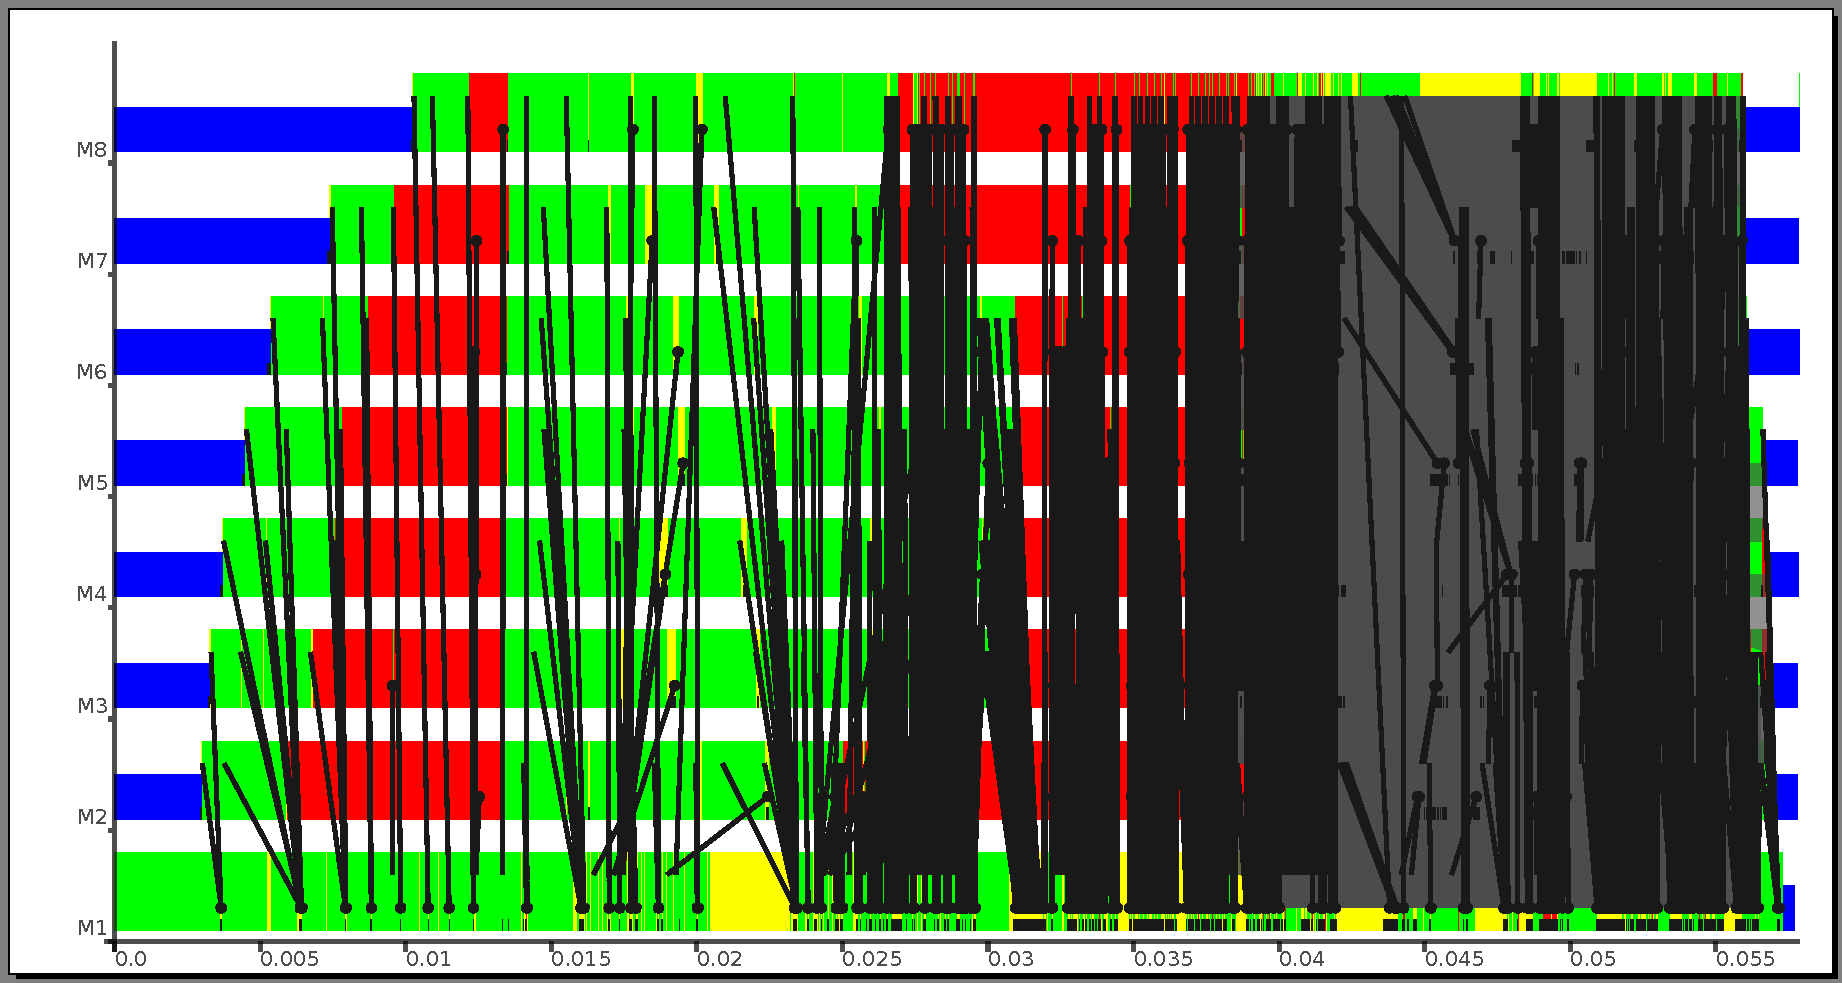
\includegraphics[width=0.9\textwidth]{images/torus_matrix_parrows_scale}
	\caption[Matrix multiplication with |torus| (PArrows)]{Matrix multiplication with |torus| (PArrows).}
	\label{fig:torus_parrows_trace}
\end{figure}

\begin{figure}[tb]
	\centering
	\includegraphics[width=0.9\textwidth]{images/torus_matrix_eden_scale}
	\caption[Matrix multiplication with |torus| (Eden)]{Matrix multiplication with |torus| (Eden).}
	\label{fig:torus_eden_trace}
\end{figure}

%\FloatBarrier

%%% Local Variables:
%%% mode: latex
%%% TeX-master: "main"
%%% End:

	\AtBeginSection{}
	\bibliography{../paper/references}
	\section{Further Notes}
	\begin{frame}[fragile]{Profit}
So... What does this get us?\\~\\
\begin{itemize}
	\item Arrow based Haskell $\Rightarrow$ \textbf{Free Parallelism} for (other) Arrows
	\item \textbf{Replaceable Backends} $\Rightarrow$ Easier Development
	\item possible \textbf{common interface} for parallelism benchmarks
	\item Arrows are quite \textbf{intuitive} for parallelism
\end{itemize}
\vfill	
\end{frame}
	\begin{frame}[fragile]{Further information}
	\begin{minipage}{0.6\textwidth}
	Paper submission:\\
	\url{https://arxiv.org/pdf/1801.02216.pdf}\\~\\
	GitHub repository:\\
	\url{https://github.com/s4ke/Parrows}\\~\\
	Frege Version in the works:\\
	\url{https://goo.gl/oHbqh0}
	\end{minipage}
	\hfill
	\begin{minipage}{0.3\textwidth}
		\begin{center}
			\vspace{0.5cm}
			
\includegraphics[scale=0.025]{images/haskell-logo}\\
			\vspace{0.3cm}
			\includegraphics[scale=0.1]{images/GitHub-Mark}\\
			\vspace{0.3cm}
			
\includegraphics[scale=0.1]{images/frege-logo}
		\end{center}
		\vfill
	\end{minipage}	
\end{frame}
	\appendix
	\begin{frame}[fragile]{Functional Programming 101}
\begin{minipage}{0.5\textwidth}
\begin{lstlisting}[frame=htrbl, language=java]
public static int fib(int x) {
	if (x<=0)
		return 0;
	else if (x==1)
		return 1;
	else
		return fib(x-2) + fib(x-1);
}
\end{lstlisting}
\end{minipage}
\hfill
\begin{minipage}{0.4\textwidth}
\begin{lstlisting}[frame=htrbl]
fib :: Int -> Int
fib x
	| x <= 0 = 0
	| x == 1 = 0
	| otherwise = 
		(fib (x - 2))
			+ (fib (x - 1))
\end{lstlisting}
\end{minipage}

\begin{itemize}
\item Functional programming equally powerful as imperative programming

\item focused on the "what?" instead of the "how?"

$\Rightarrow$ more concise $\Rightarrow$ easier to reason about

\item based on Lambda Calculus
\end{itemize}
\end{frame}
	\begin{frame}[fragile]{pipe2}
\begin{lstlisting}[frame=htrbl, language=java]
pipe2 :: conf -> arr a b -> arr b c -> arr a c
pipe2 conf f g =
    (arr return &&& arr (const [])) &&& arr (const []) >>>
    pipe conf (replicate 2 (unify f g)) >>>
    arr snd >>>
    arr head
    where
        unify :: arr a b -> arr b c -> 
            arr (([a], [b]), [c]) (([a], [b]), [c])
        unify f' g' = (mapArr f' *** mapArr g') *** arr (const [])
            >>> arr (\((b, c), a) -> ((a, b), c))
\end{lstlisting}
\end{frame}

\begin{frame}[fragile]{ring}
\begin{lstlisting}[frame=htrbl, language=java]
ring :: conf -> arr (i, r) (o, r) -> arr [i] [o]
ring conf f =
    loop (second (rightRotate >>> lazy) >>>
        arr (uncurry zip) >>>
        loopParEvalN conf
            (repeat (second (get conf) >>> f >>>
                second (put conf))) >>>
        arr unzip) >>>
    postLoopParEvalN conf (repeat (arr id))
\end{lstlisting}
\end{frame}

\begin{frame}[fragile]{torus}
\begin{lstlisting}[frame=htrbl, language=java]
torus :: conf -> arr (c, a, b) (d, a, b) -> arr [[c]] [[d]]
torus conf f =
    loop (second ((mapArr rightRotate >>> lazy)
            *** (arr rightRotate >>> lazy)) >>>
        arr (uncurry3 (zipWith3 lazyzip3)) >>>
        arr length &&& (shuffle >>>
            loopParEvalN conf (repeat (ptorus conf f))) >>>
        arr (uncurry unshuffle) >>>
        arr (map unzip3) >>> arr unzip3 >>> threetotwo) >>>
    postLoopParEvalN conf (repeat (arr id))
\end{lstlisting}
\end{frame}
\end{document}